% -*- TeX:RNW:UK -*-
\documentclass[10pt]{beamer}\usepackage[]{graphicx}\usepackage[]{color}
% maxwidth is the original width if it is less than linewidth
% otherwise use linewidth (to make sure the graphics do not exceed the margin)
\makeatletter
\def\maxwidth{ %
  \ifdim\Gin@nat@width>\linewidth
    \linewidth
  \else
    \Gin@nat@width
  \fi
}
\makeatother

\definecolor{fgcolor}{rgb}{0.345, 0.345, 0.345}
\makeatletter
\@ifundefined{AddToHook}{}{\AddToHook{package/xcolor/after}{\definecolor{fgcolor}{rgb}{0.345, 0.345, 0.345}}}
\makeatother
\newcommand{\hlnum}[1]{\textcolor[rgb]{0.686,0.059,0.569}{#1}}%
\newcommand{\hlstr}[1]{\textcolor[rgb]{0.192,0.494,0.8}{#1}}%
\newcommand{\hlcom}[1]{\textcolor[rgb]{0.678,0.584,0.686}{\textit{#1}}}%
\newcommand{\hlopt}[1]{\textcolor[rgb]{0,0,0}{#1}}%
\newcommand{\hlstd}[1]{\textcolor[rgb]{0.345,0.345,0.345}{#1}}%
\newcommand{\hlkwa}[1]{\textcolor[rgb]{0.161,0.373,0.58}{\textbf{#1}}}%
\newcommand{\hlkwb}[1]{\textcolor[rgb]{0.69,0.353,0.396}{#1}}%
\newcommand{\hlkwc}[1]{\textcolor[rgb]{0.333,0.667,0.333}{#1}}%
\newcommand{\hlkwd}[1]{\textcolor[rgb]{0.737,0.353,0.396}{\textbf{#1}}}%
\let\hlipl\hlkwb

\usepackage{framed}
\makeatletter
\newenvironment{kframe}{%
 \def\at@end@of@kframe{}%
 \ifinner\ifhmode%
  \def\at@end@of@kframe{\end{minipage}}%
  \begin{minipage}{\columnwidth}%
 \fi\fi%
 \def\FrameCommand##1{\hskip\@totalleftmargin \hskip-\fboxsep
 \colorbox{shadecolor}{##1}\hskip-\fboxsep
     % There is no \\@totalrightmargin, so:
     \hskip-\linewidth \hskip-\@totalleftmargin \hskip\columnwidth}%
 \MakeFramed {\advance\hsize-\width
   \@totalleftmargin\z@ \linewidth\hsize
   \@setminipage}}%
 {\par\unskip\endMakeFramed%
 \at@end@of@kframe}
\makeatother

\definecolor{shadecolor}{rgb}{.97, .97, .97}
\definecolor{messagecolor}{rgb}{0, 0, 0}
\definecolor{warningcolor}{rgb}{1, 0, 1}
\definecolor{errorcolor}{rgb}{1, 0, 0}
\makeatletter
\@ifundefined{AddToHook}{}{\AddToHook{package/xcolor/after}{
\definecolor{shadecolor}{rgb}{.97, .97, .97}
\definecolor{messagecolor}{rgb}{0, 0, 0}
\definecolor{warningcolor}{rgb}{1, 0, 1}
\definecolor{errorcolor}{rgb}{1, 0, 0}
}}
\makeatother
\newenvironment{knitrout}{}{} % an empty environment to be redefined in TeX

\usepackage{alltt}
\usetheme{metropolis}
%\useinnertheme{rectangles}
\setbeamercovered{%
still covered={\opaqueness<1->{15}},
again covered={\opaqueness<1->{40}}}

\hypersetup{colorlinks,linkcolor=black,urlcolor=brown,citecolor=brown}

\usepackage{amsmath,amssymb,amsthm}
\usepackage{unicode-math}

% We set the Lucida OTF fonts as default
\usepackage{fontspec}
\setmainfont{Lucida Bright OT}
\setsansfont{Lucida Sans OT}
\setmonofont{Lucida Console DK}[Scale=MatchLowercase]

\newfontfamily\webglyphsfont{WebHostingHub-Glyphs}[Scale=0.7]
\newcommand\webglyphs[1]{{\webglyphsfont\symbol{#1}}}
\newcommand\Discussion{\colorbox{white}{\textcolor{black}{\webglyphs{"F134}}}\xspace}
\newcommand\DiscussionI{\colorbox{black}{\textcolor{white}{\webglyphs{"F134}}}\xspace}
\newcommand\DExamples{\colorbox{black}{\textcolor{white}{\webglyphs{"F134} examples?}}}
\newcommand\Reading{\colorbox{black}{\textcolor{white}{\webglyphs{"F0C1}}}\xspace}
\newcommand\ReadingI{\colorbox{white}{\textcolor{black}{\webglyphs{"F0C1}}}\xspace}
\newcommand\Video{\colorbox{white}{\textcolor{black}{\webglyphs{"F03D}}}\xspace}
\newcommand\Attention{\colorbox{black}{\textcolor{orange}{\webglyphs{"F05A}}}\xspace}
\newcommand\HomeWork{\colorbox{white}{\textcolor{black}{\webglyphs{"F5ED}}}\xspace}
\newcommand\HomeWorkI{\colorbox{black}{\textcolor{white}{\webglyphs{"F5ED}}}\xspace}
\newcommand\Advanced{\colorbox{black}{\textcolor{white}{\webglyphs{"F235}}}\xspace}

\newfontfamily\lineabasicfont{linea-basic-10}
\newcommand\basicicons[1]{{\lineabasicfont\symbol{#1}}}
\newcommand\timeforwards{\basicicons{"0079}}
\newcommand\timebackwards{\basicicons{"0064}}

\newfontfamily\lineaweatherfont{linea-weather-10}
\newcommand\weathericons[1]{{\lineaweatherfont\symbol{#1}}}
\newcommand\meteosun{\weathericons{"E038}}
\newcommand\meteosuncloud{\weathericons{"E042}}
\newcommand\meteorain{\weathericons{"E033}}
\newcommand\meteowind{\weathericons{"E054}}

\newfontfamily\uleaffont{Mini Pics Uprooted Leaf}
\newcommand\uleafmpics[1]{{\uleaffont\symbol{#1}}}
\newcommand\lowplants{\uleafmpics{"00CE}}
\newcommand\mediumplant{\uleafmpics{"006A}}
\newcommand\bush{\uleafmpics{"0039}}
\newcommand\smallplant{\uleafmpics{"0030}}
\newcommand\seedling{\uleafmpics{"002F}}
\newcommand\floweringplant{\uleafmpics{"00CA}}

\newfontfamily\utwigfont{Mini Pics Uprooted Twig}
\newcommand\utwigmpics[1]{{\utwigfont\symbol{#1}}}
\newcommand\grassplant{\utwigmpics{"0033}}

\newfontfamily\uinsectfont{Insect Icons}
\newcommand\uinsect[1]{{\uinsectfont\symbol{#1}}}
\newcommand\bug{\uinsect{"006F}}

\usepackage{polyglossia}
\setdefaultlanguage[variant = british, ordinalmonthday = false]{english}

\usepackage[style=authoryear-comp,firstinits,sortcites,maxcitenames=2,%
    mincitenames=1,maxbibnames=10,minbibnames=10,uniquename=mininit,%
    uniquelist=minyear,sortfirstinits=true]{biblatex}
\addbibresource{../references/ecophys.bib}
\renewcommand{\bibfont}{\small}

\usepackage{abbrev}


\IfFileExists{upquote.sty}{\usepackage{upquote}}{}
\begin{document}





\title{PBIO-141\\Sensory and Physiological Ecology of  Plants}
\subtitle{4: The Light Environment}
\author{Pedro J. Aphalo}
\date{January--February 2022}
\institute[Univ.\ of Helsinki]{M.Sc.\ in Plant Biology, University of Helsinki\\[2ex] \url{http://blogs.helsinki.fi/aphalo/}}

  \begin{frame}
    \maketitle
  \end{frame}

  \begin{frame}[c]
    \begin{center}
      \begin{small}
        \copyright 2006--2022 by Pedro J. Aphalo\\
        University of Helsinki, Finland.\\
        \textcolor{blue}{\url{http://blogs.helsinki.fi/senpep-blog/}}\\[2ex]
      \end{small}

      \begin{footnotesize}
        Sensory and Physiological Ecology of Plants slides by Pedro J. Aphalo are licensed under a Creative Commons Attribution-ShareAlike 4.0 International License.

      
\includegraphics[width=6em]{../figures/copyright/by-sa}\\[2ex]
      \end{footnotesize}
        
        \begin{scriptsize}
        Typeset in Lucida Sans, \textrm{Luicda Bright}, \texttt{Lucida Console} and Lucida Math. Icons from fonts ``WebHostingHub Glyphs'' (under SIL-Open Font License) from \url{https://www.webhostinghub.com/}; ``insect icons'' (free from \url{http://www.woodcutter.es/}); ``linea-basic-10'' and ``linea-weather-10'' (free from \url{https://github.com/linea-io}), ``Mini Pics Uprooted Twig'' and ``Mini Pics Uprooted Twig'' (commercial, from Image Club Graphics, Inc.). Plant icon as .svg by Abdul Wahhab (free from \url{NounProject.com}).

        Illustrations and text quoted from copyrighted sources is excluded from this license and their use should respect the original licenses.
        \end{scriptsize}
    \end{center}
  \end{frame}


  \begin{frame}
    \frametitle{Outline}
    \tableofcontents
  \end{frame}

\section{Solar radiation}

\begin{frame}{Radiation: properties}
    \begin{itemize}
        \item Wavelength ($\lambda$), perceived by humans as `colours'.
        \item Direction: one direction (`collimated'), many directions (`diffuse').
        \begin{itemize}
            \item Direct solar radiation: radiation arriving directly from the
            sun.
            \item Diffuse solar radiation: solar radiation scattered by the
            atmosphere or reflected by clouds.
            \item Global radiation: direct radiation + diffuse radiation.
        \end{itemize}
        \item Duration: `length of time' (e.g.\ day length, or sunfleck frequency).
        \item Other: polarization, etc.
    \end{itemize}
\end{frame}

\begin{frame}{Radiation: quantities and units}
    \begin{description}
        \item[Irradiance:] flux of radiation received at a flat
        surface.
        \item[Energy irradiance:] irradiance expressed as energy per
        unit area and unit time. Units: J s$^{-1}$ m$^{-2}$ = W m$^{-2}$.
        \item[Photon irradiance:] irradiance expressed as number of
        photons per unit area and unit time. Units: mol s$^{-1}$ m$^{-2}$.
        \item[Spectral photon irradiance:] Irradiance measured over a
        narrow band, expressed as number of photons per unit area
        and unit time and waveband. Units: mol s$^{-1}$ m$^{-2}$ nm$^{-1}$.
%        \item[Photosynthetic photon flux density (PPFD):]<5> Another name
%        for PAR photon irradiance.
    \end{description}
\end{frame}

\begin{frame}{Radiation: Cosine law}
    \centering
    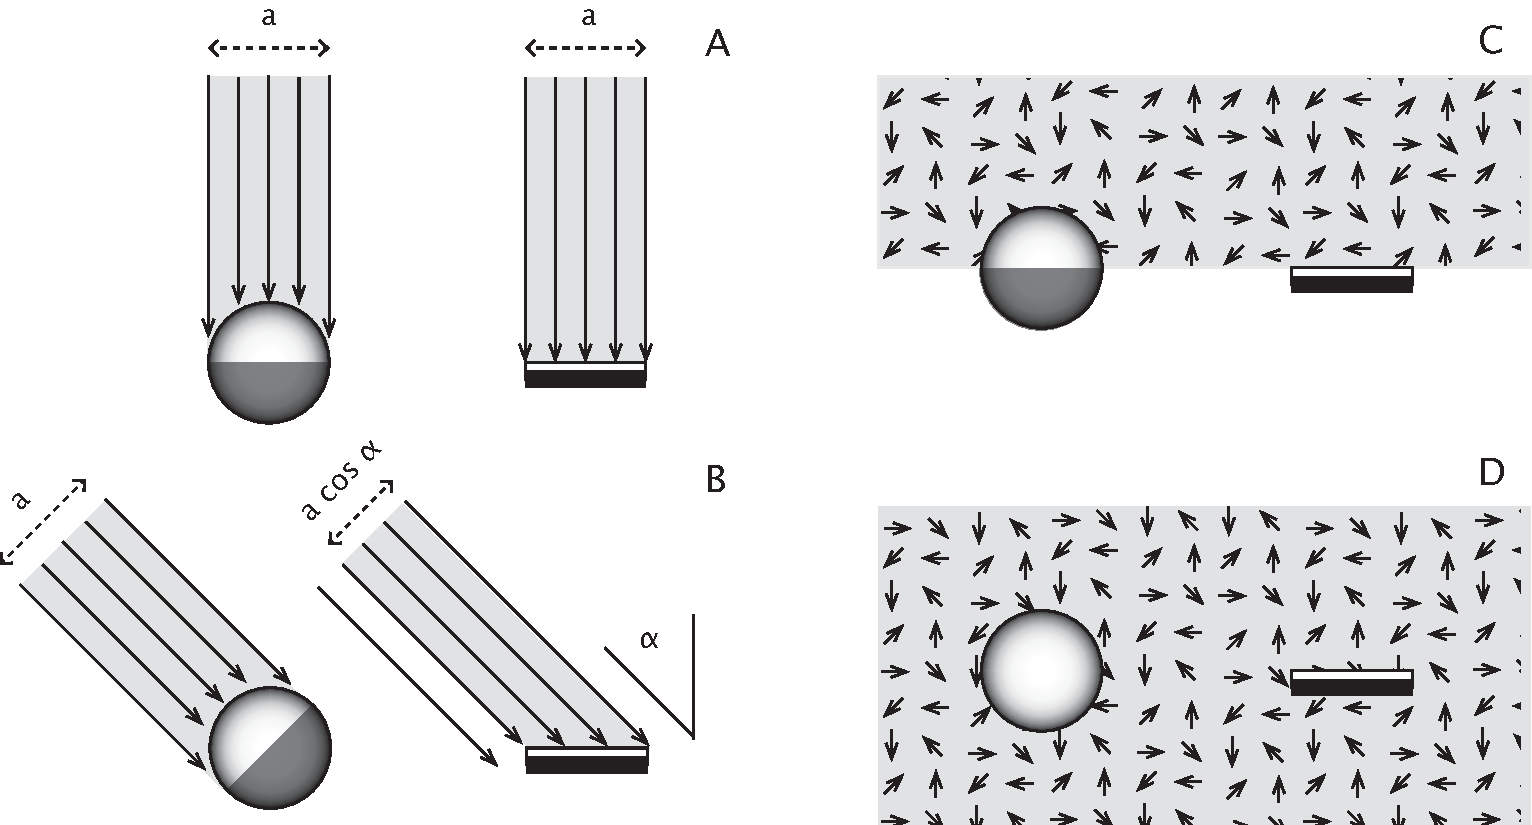
\includegraphics[width=0.9\textwidth]{figures/cosine_arrows}

    {\small Irradiance on a surface depends on the angle of incidence
    \autocite[from][]{Aphalo2012}}
\end{frame}

\begin{frame}{Optical radiation or light colour}

\begin{knitrout}\tiny
\definecolor{shadecolor}{rgb}{0.969, 0.969, 0.969}\color{fgcolor}

{\centering \includegraphics[width=0.97\textwidth]{figure/pos-wavebans-1} 

}


\end{knitrout}
\end{frame}

\begin{frame}{Radiation: wavelength ranges of `colours'}
    \begin{description}
        \item[Shortwave radiation] $\lambda <$ 4\,000 nm (4 $\mymu$m).
        \item[Longwave radiation] $\lambda >$ 4\,000 nm (4 $\mymu$m).
        \item[Ultraviolet radiation] 100 nm $ < \lambda <$ 400 nm.
        \begin{description}
            \item[UV-C] 100 nm $< \lambda <$ 280 nm.
            \item[UV-B] 280 nm $< \lambda <$ 315 nm.
            \item[UV-A1] 315 nm $< \lambda <$ 340 nm.
            \item[UV-A2] 340 nm $< \lambda <$ 400 nm.
        \end{description}
        \item[VIS] light, `visible to humans' 380 nm $< \lambda <$ 760~nm.
        \item[PAR] `useful for photosynthesis' 400 nm $< \lambda <$ 700 nm.
        \item[Far red (FR)] 700 nm $< \lambda <$ 750--800 nm.
        \item[Infrared (IR)] `thermal' approx.\ 750 nm $< \lambda <$ 1 mm.
    \end{description}
    \small{$\lambda$: wavelength.}
\end{frame}

\begin{frame}
  \frametitle{Solar radiation spectrum: photon units}

  \textbf{In Viikki, midsummer day, noon, partly cloudy.}

\begin{knitrout}\tiny
\definecolor{shadecolor}{rgb}{0.969, 0.969, 0.969}\color{fgcolor}

{\centering \includegraphics[width=0.97\textwidth]{figure/pos-solar-spectrum-q-1} 

}


\end{knitrout}
\end{frame}

\begin{frame}
  \frametitle{Solar radiation spectrum: energy units}

  \textbf{In Viikki, midsummer day, noon, partly cloudy.}

\begin{knitrout}\tiny
\definecolor{shadecolor}{rgb}{0.969, 0.969, 0.969}\color{fgcolor}

{\centering \includegraphics[width=0.97\textwidth]{figure/pos-solar-spectrum-e-1} 

}


\end{knitrout}
\end{frame}



\begin{frame}
  \frametitle{Solar radiation (PAR, 400 nm to 700 nm)}

  \textbf{In Viikki, one day in summer, almost no clouds}.
  
  Total PAR (yellow) and diffuse (blue) PAR.

\begin{knitrout}\tiny
\definecolor{shadecolor}{rgb}{0.969, 0.969, 0.969}\color{fgcolor}

{\centering \includegraphics[width=0.97\textwidth]{figure/pos-solar-irrad-Viiki_clear-1} 

}


\end{knitrout}
\end{frame}

\begin{frame}
  \frametitle{Solar radiation (PAR)}

  \textbf{In Viikki, in summer, broken clouds.}

  Total PAR (yellow) and diffuse (blue) PAR.

\begin{knitrout}\tiny
\definecolor{shadecolor}{rgb}{0.969, 0.969, 0.969}\color{fgcolor}

{\centering \includegraphics[width=0.97\textwidth]{figure/pos-solar-irrad-Viiki-clouds-1} 

}


\end{knitrout}
\end{frame}

\begin{frame}
  \frametitle{Solar radiation (PAR)}

  \textbf{In Viikki, in summer, overcast.}

  Total PAR (yellow) and diffuse (blue) PAR.

\begin{knitrout}\tiny
\definecolor{shadecolor}{rgb}{0.969, 0.969, 0.969}\color{fgcolor}

{\centering \includegraphics[width=0.97\textwidth]{figure/pos-solar-irrad-Viiki-overcast-1} 

}


\end{knitrout}
\end{frame}

\begin{frame}{Diffuse sunlight and wavelength: UV and NIR}
  \centering
  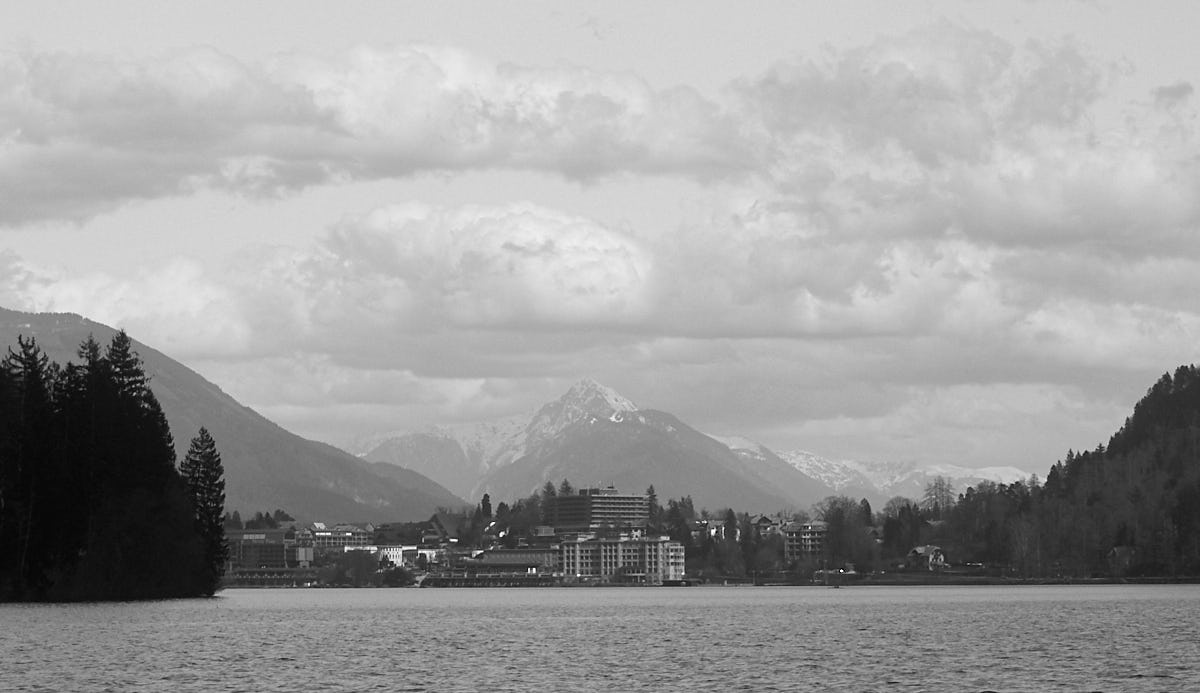
\includegraphics[height = 0.44\textheight]{photos/Bled-UVA}\\
  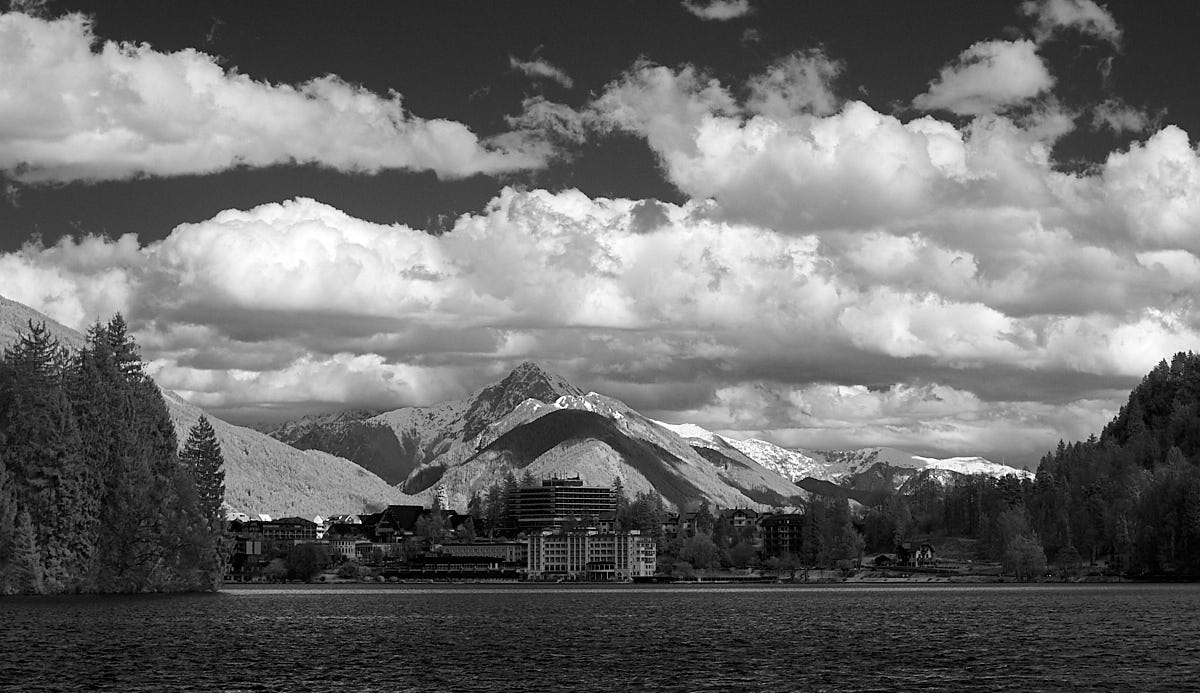
\includegraphics[height = 0.44\textheight]{photos/Bled-NIR}
\end{frame}

\begin{frame}{Light environment \Discussion}
\begin{block}{How does it change? \Discussion 10 min}
    \begin{itemize}
      \item Which properties of sunlight change with weather conditions?
      \item Which properties of sunlight change through a day?
      \item Which properties of sunlight change with seasons?
      \item Which properties of sunlight change with latitude?
      \item Which properties of sunlight change with pollution?
      \item Do plants modify light properties?
      \item Which ones?
    \end{itemize}
\end{block}

\end{frame}

\section{Radiation and leaves}

\begin{frame}{Light attenuation in leaves}

    We use the word \emph{attenuation} to mean the process by which irradiance decreases when light travels through any object.
    \vspace{1ex}

    In green leaves, light attenuation depends on:\\
    \begin{itemize}
        \item chlorophyll concentration,
        \item cuticle waxes,
        \item pubescence (trichomes or ``hairs''),
        \item mass pigments like anthocyanins, flavonoids, and other phenolics, and carotenoids,
        \item angle between the leaf and the direction of radiation.
    \end{itemize}
\end{frame}

\begin{frame}[fragile]{Transmittance, reflectance and absorptance (quantities)}

Solidago from upper canopy, light incident on adaxial (upper) epidermis.

\begin{knitrout}\tiny
\definecolor{shadecolor}{rgb}{0.969, 0.969, 0.969}\color{fgcolor}

{\centering \includegraphics[width=0.97\textwidth]{figure/pos-leaf-optics-1} 

}


\end{knitrout}

\end{frame}

\begin{frame}{Light and plant leaves}{Absorption of light}
    \begin{itemize}
        \item The absorptance of leaves for light depends on the
        wavelength.
        \item In the visible part of the spectrum they reflect and
        transmit more green light than other colours of light.
        \item A little further towards longer wavelengths, they
        reflect and transmit most of the radiation.
        \item Later in the course we will see how plants perceive
        this ratio through photoreceptors called phytochromes.
    \end{itemize}
\end{frame}

\begin{frame}{Looking at reflected far-red radiation}
%{Photographs in visible and far-red radiation ($\lambda > 715$\,nm)}
    \centering
    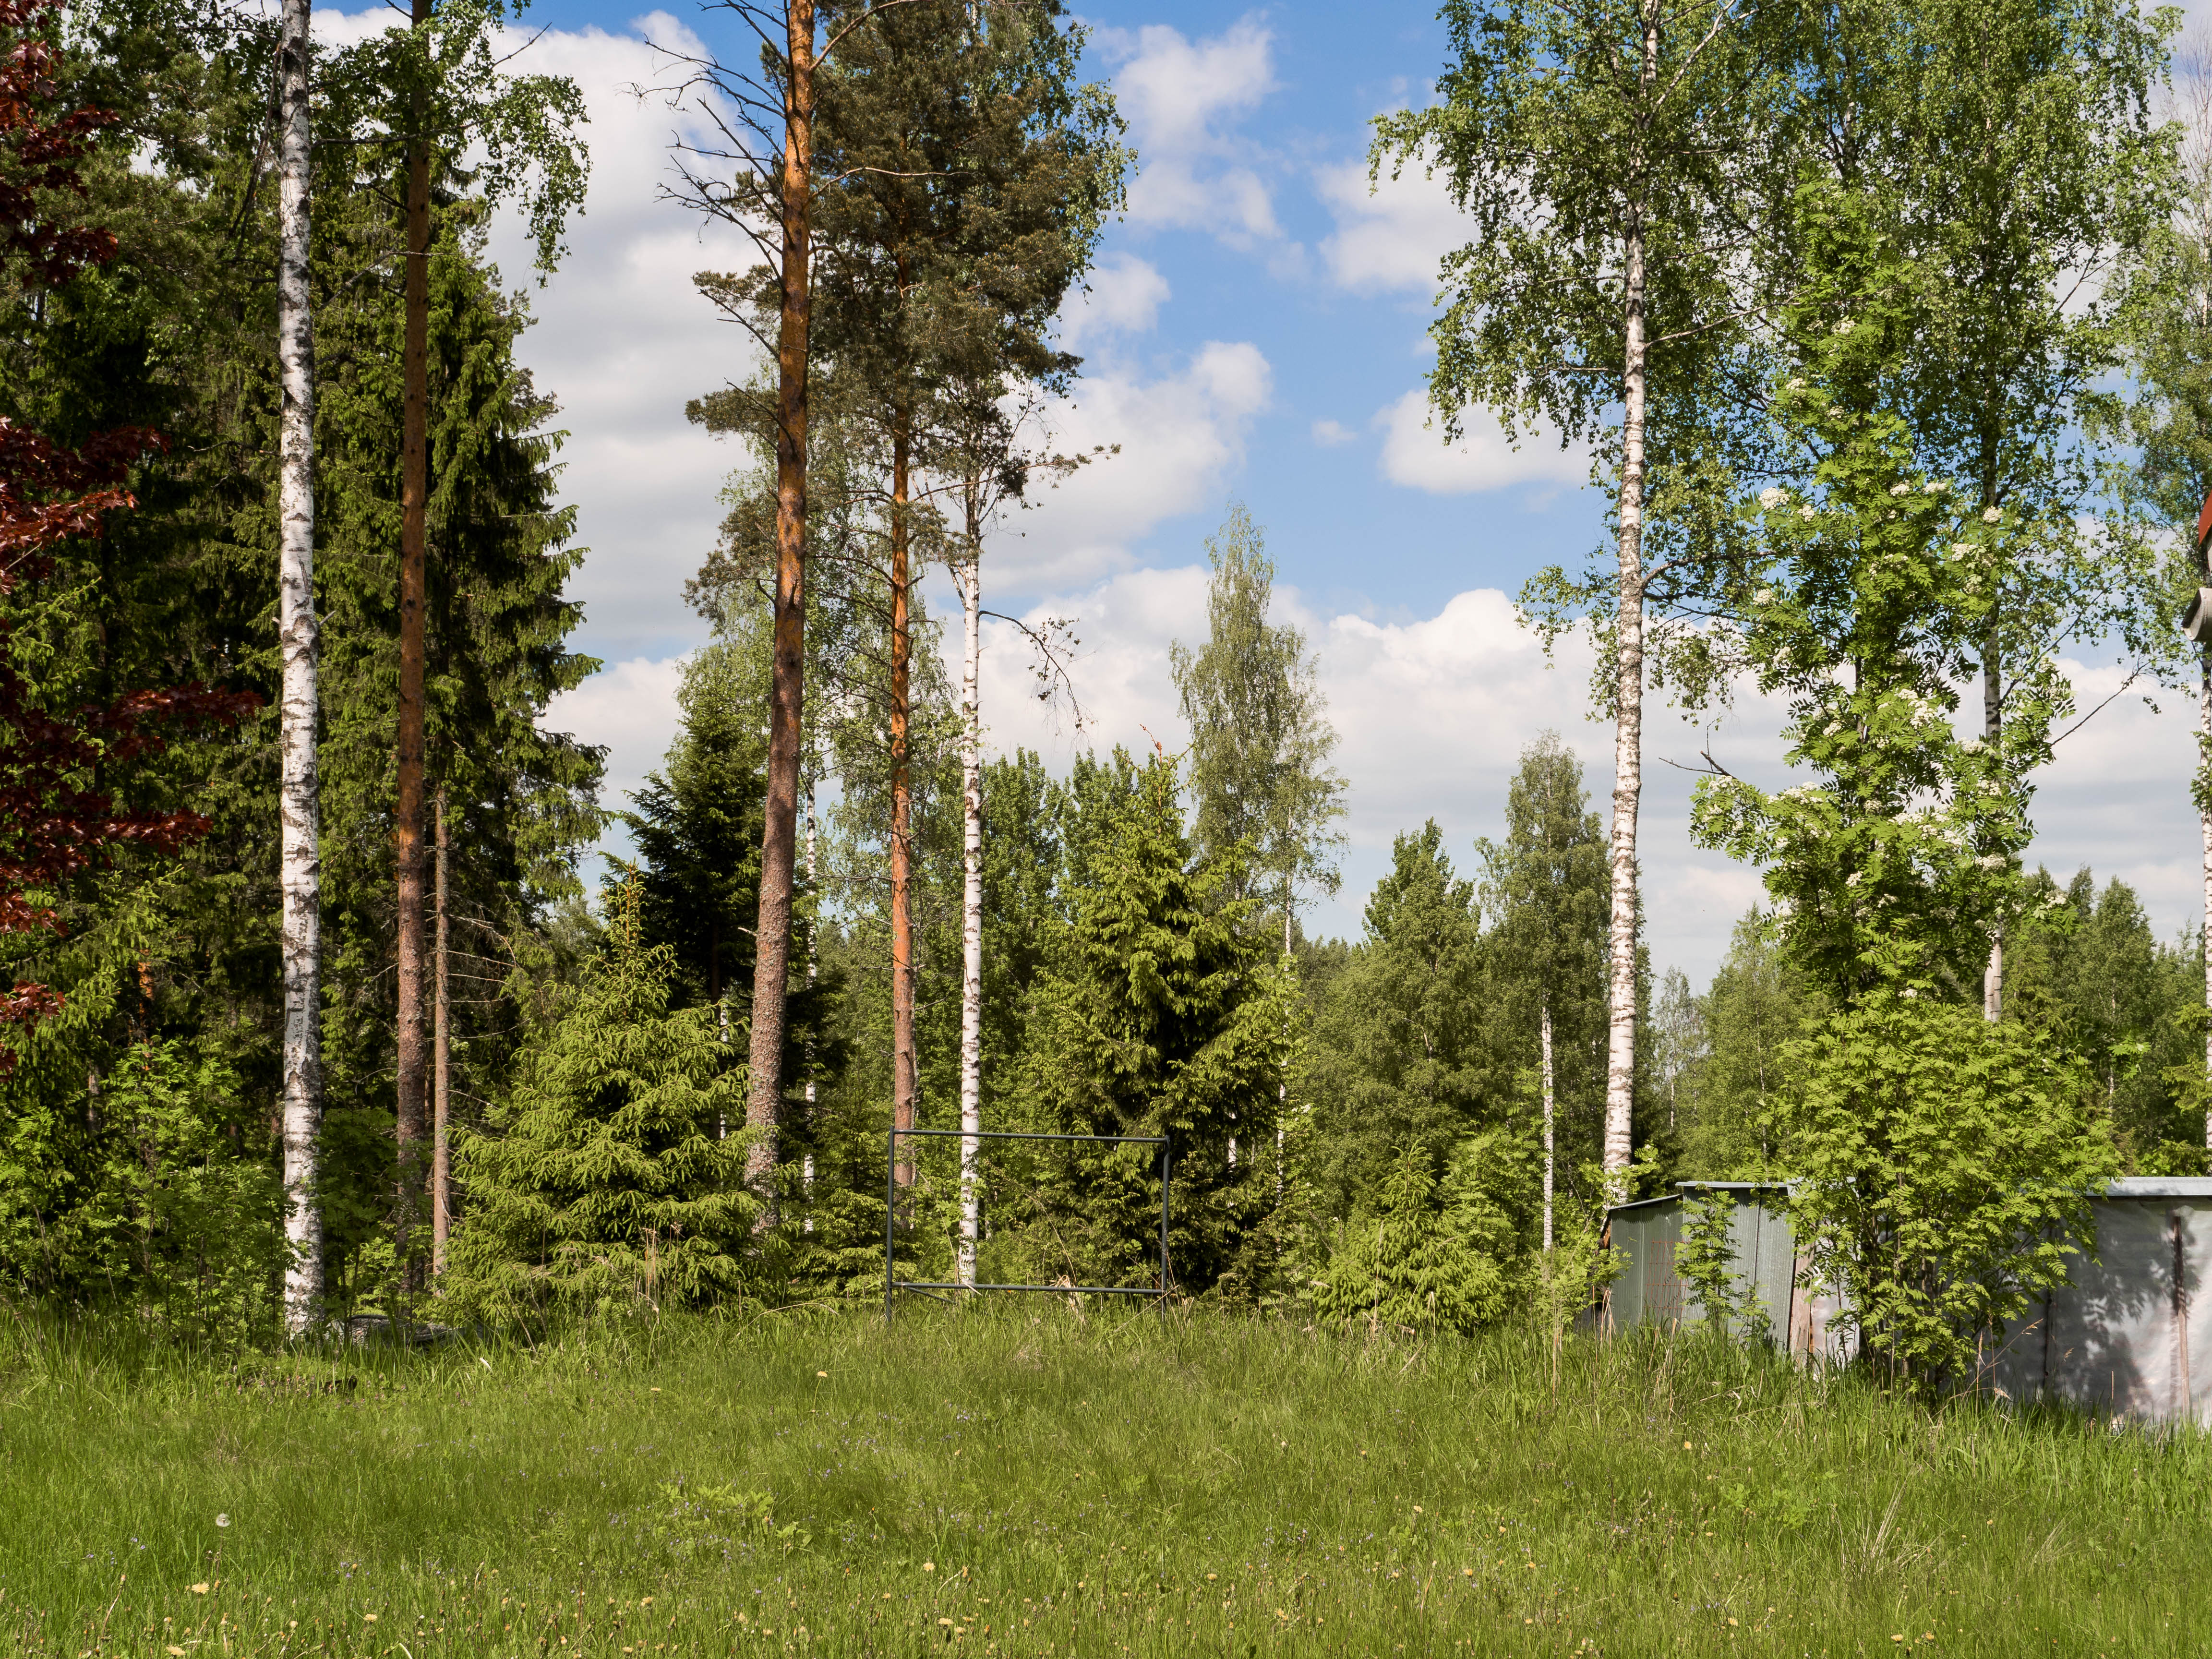
\includegraphics[width=0.45\textwidth]{photos/visible}\ %
    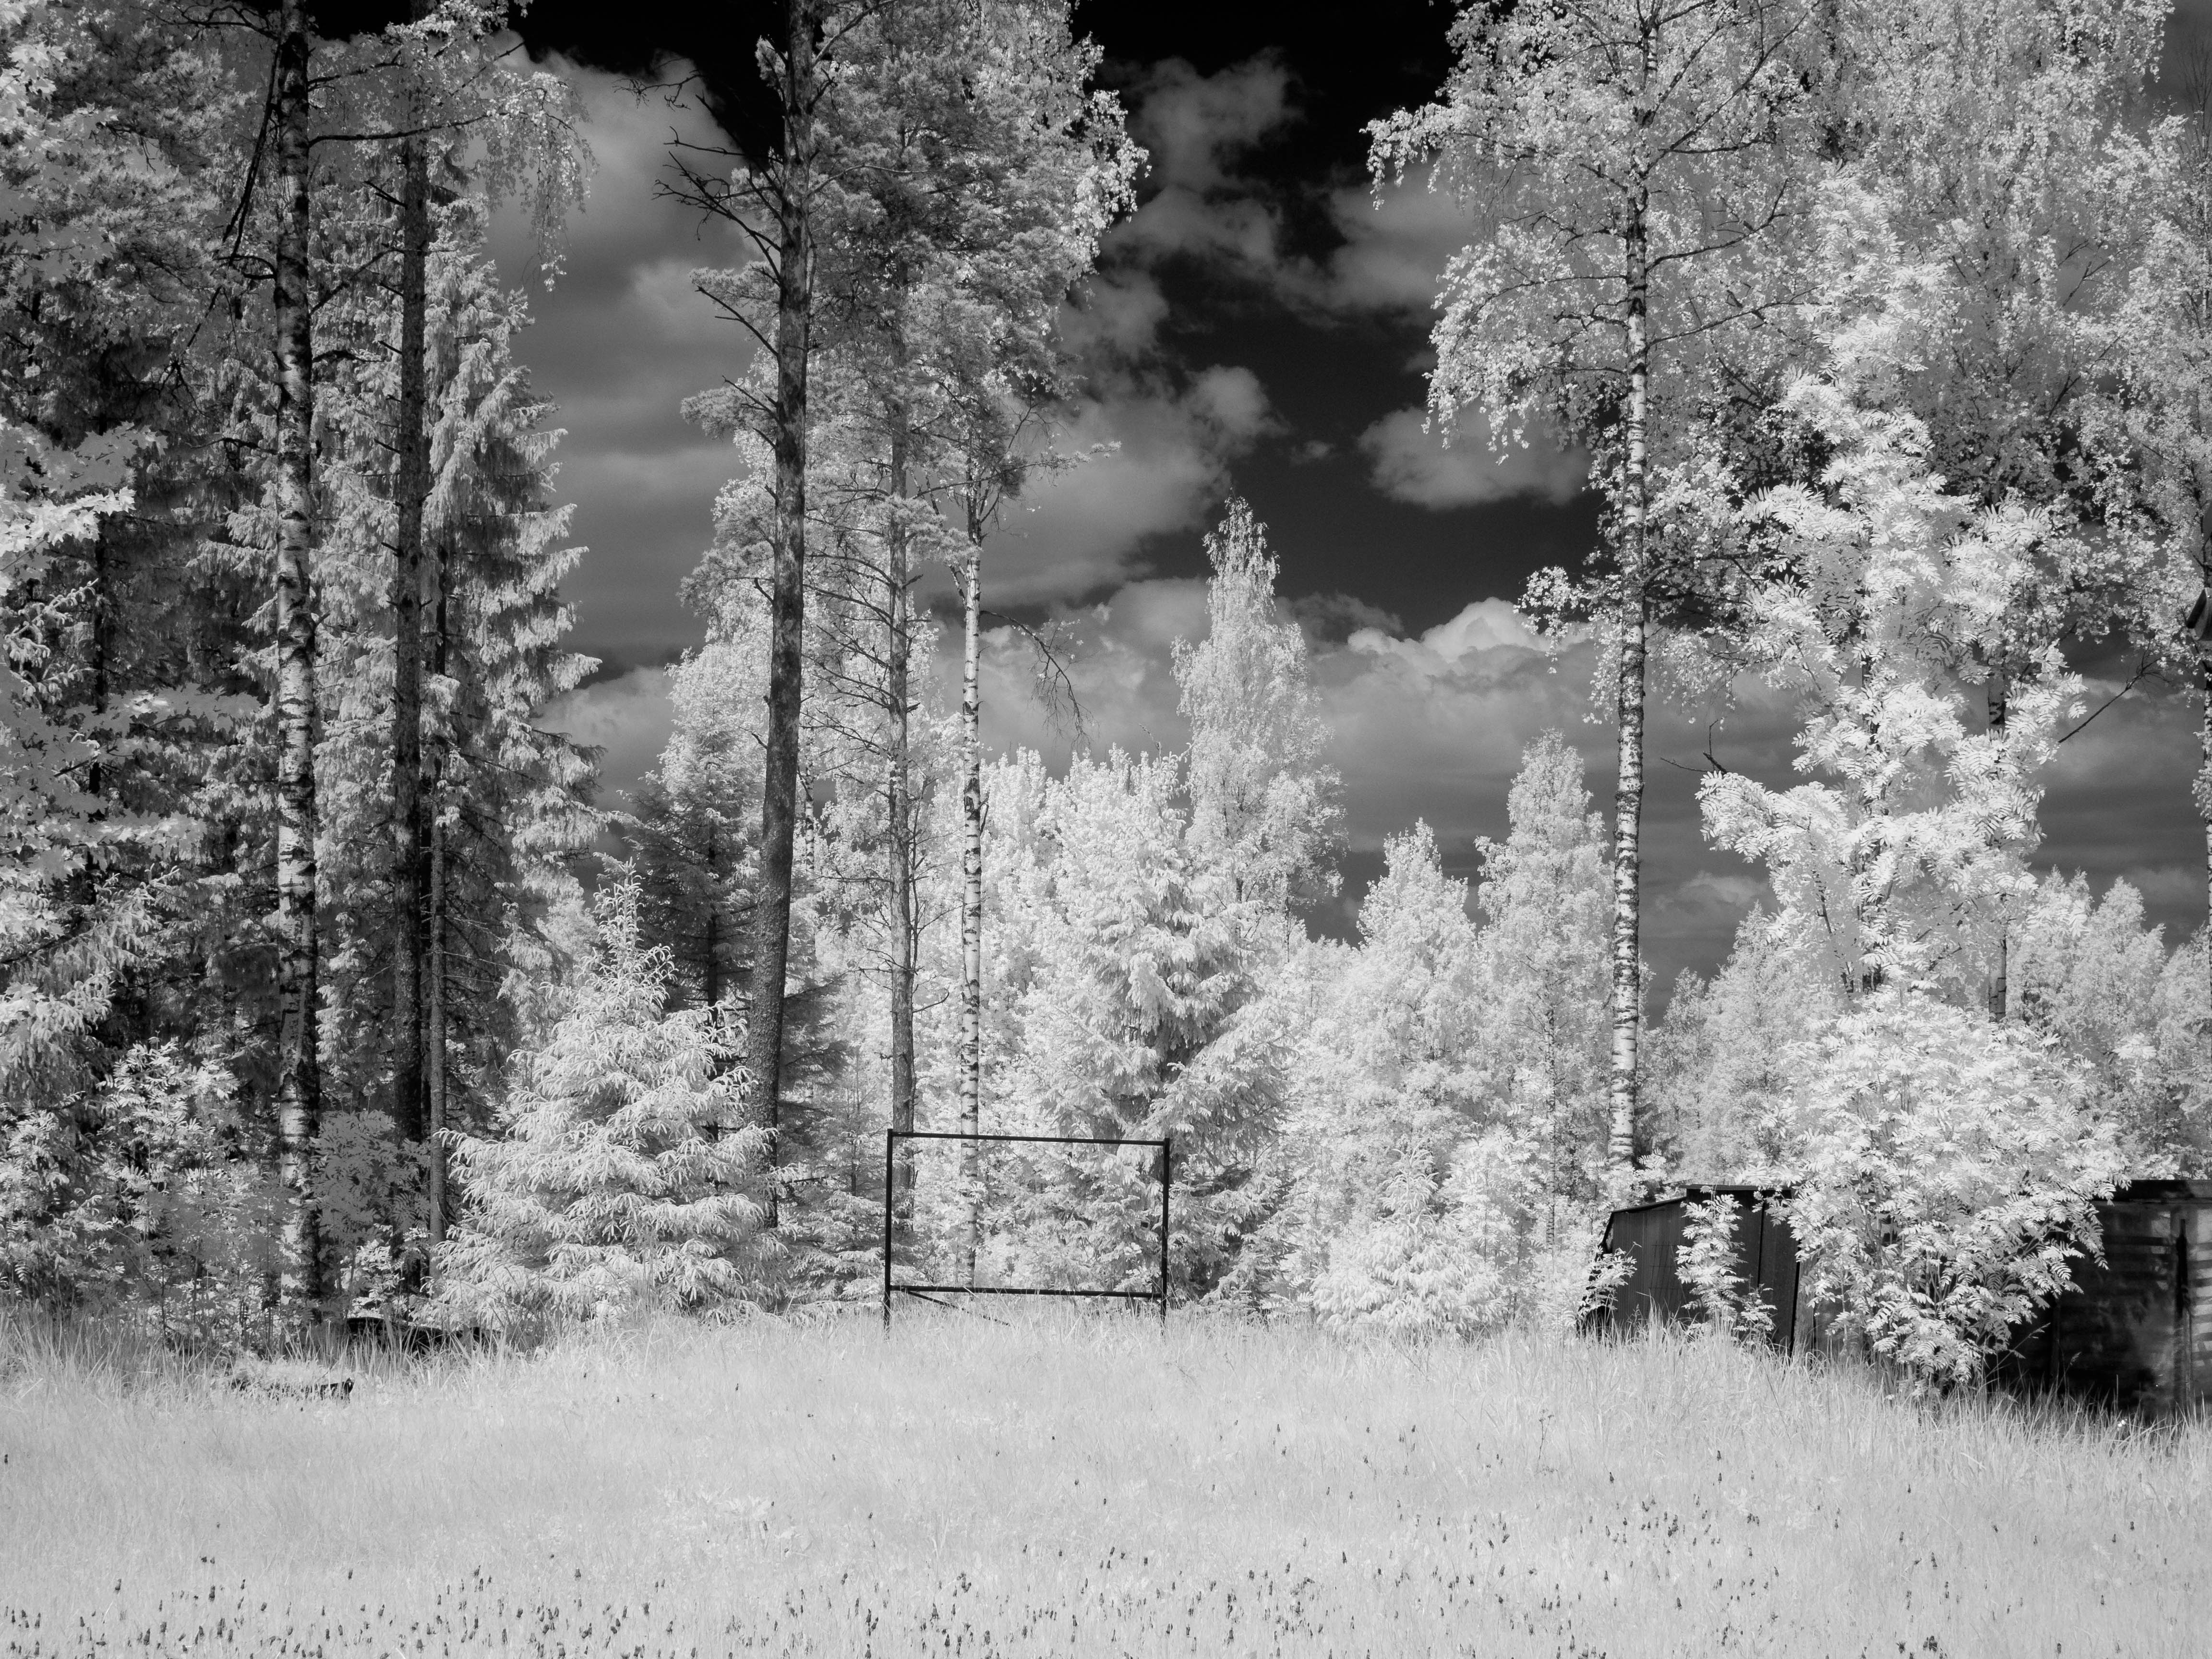
\includegraphics[width=0.45\textwidth]{photos/far-red-1}\\[0.5ex]
    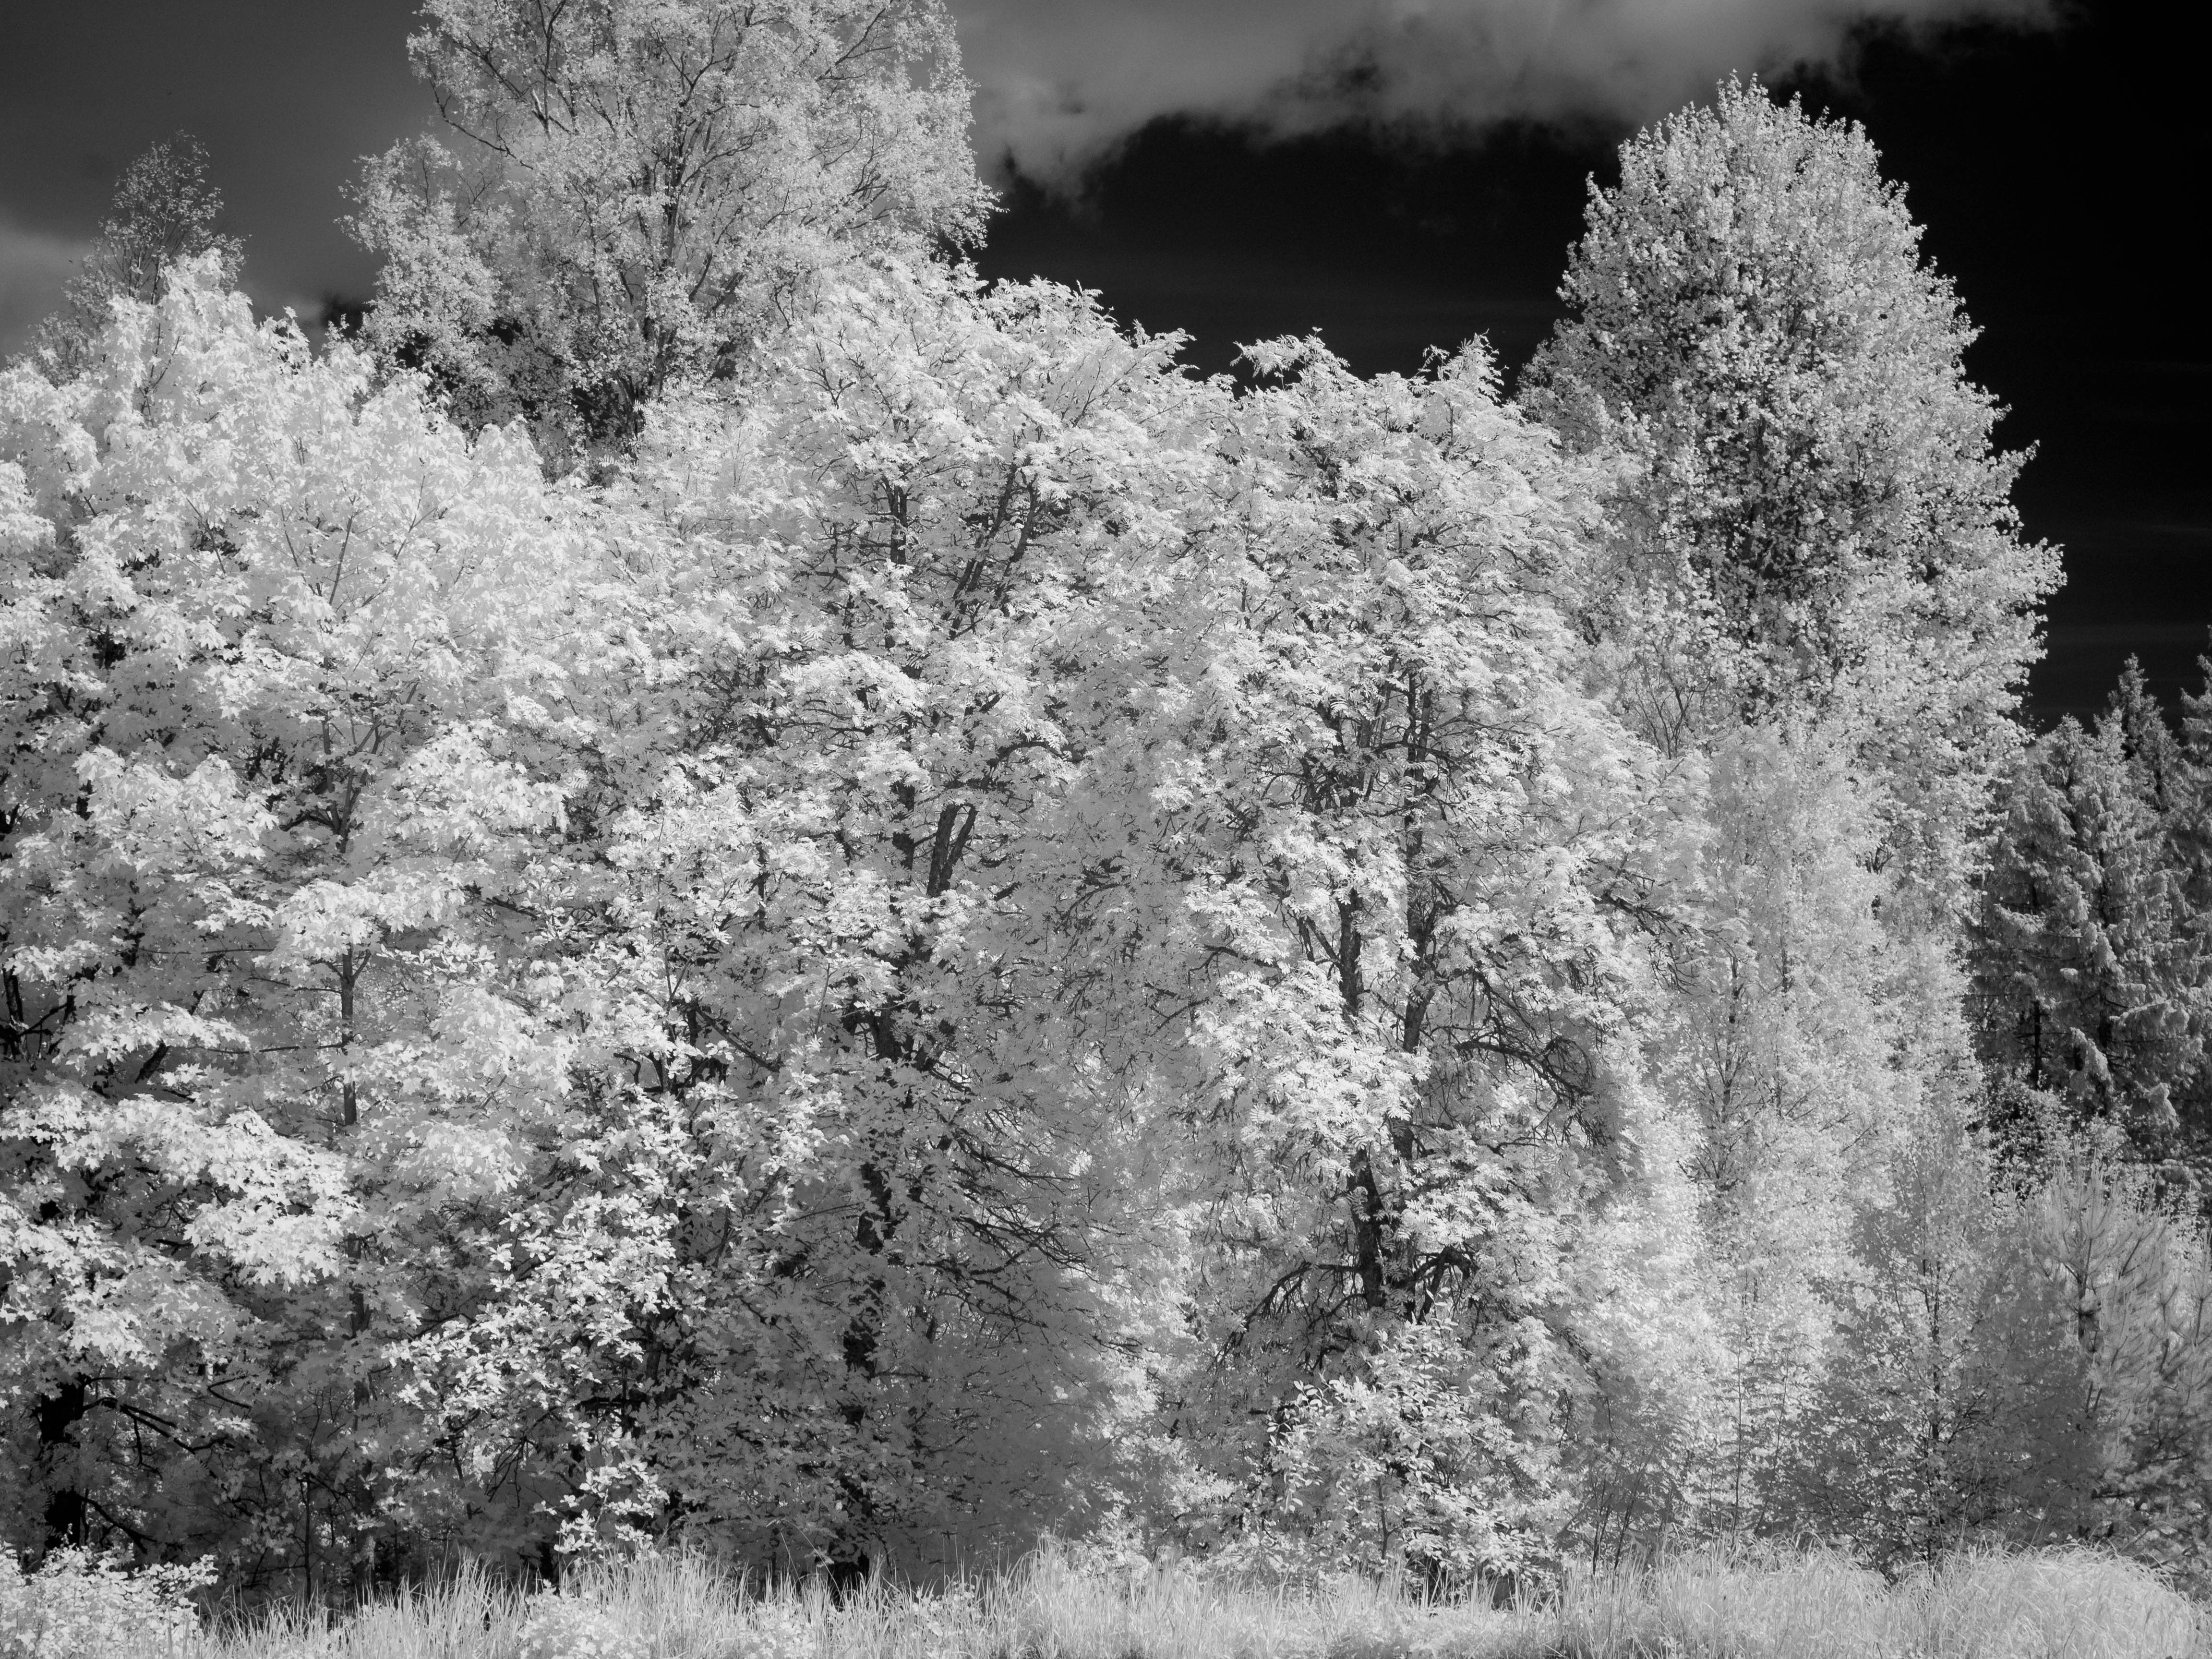
\includegraphics[height=0.45\textheight]{photos/far-red-2}\ %
    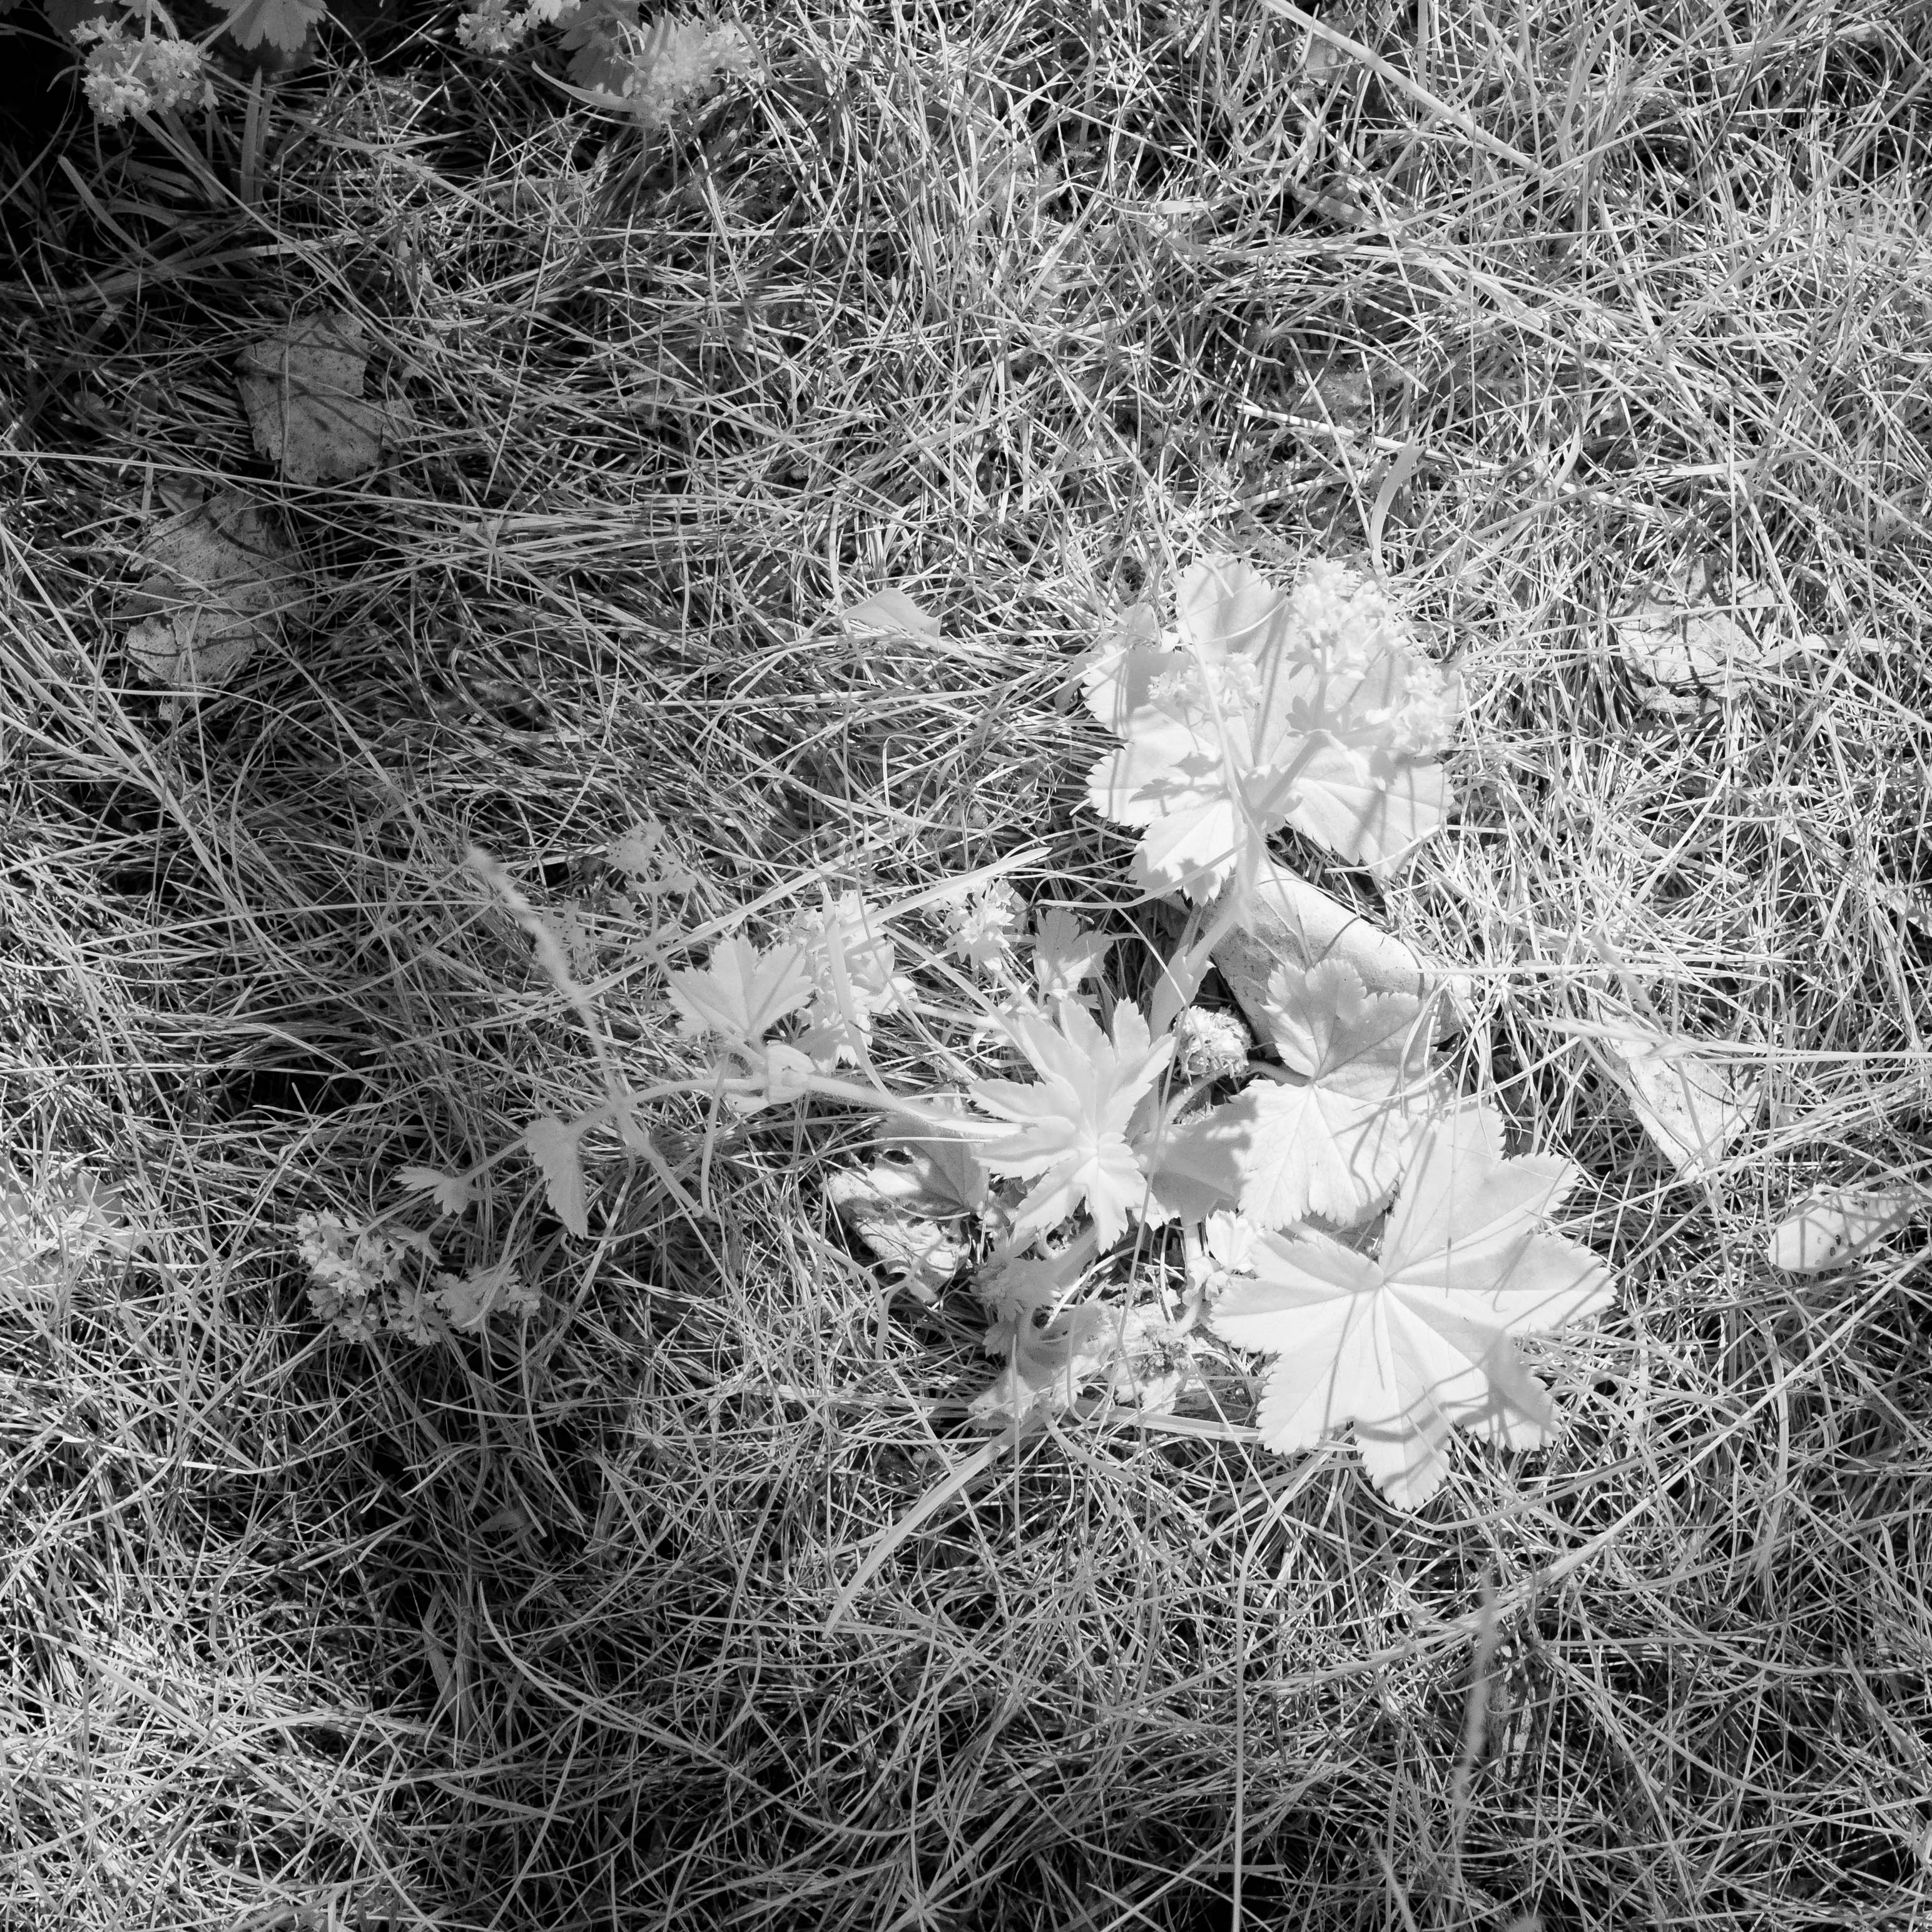
\includegraphics[height=0.45\textheight]{photos/far-red-3}

\end{frame}

\begin{frame}{Flower patterns in ultraviolet-A}
    \centering
    \includegraphics[width=0.45\textwidth]{photos/taraxacum-vis}\ %
    \includegraphics[width=0.45\textwidth]{photos/taraxacum-uva}\\

\end{frame}

\section{Radiation in plant canopies}

\begin{frame}{Light in plant canopies}{Attenuation (process)}

    We use the word \emph{attenuation} to mean the decrease in
    irradiance that occurs when light travels through any object.
    \vspace{0.04\textheight}

    In the case of canopies, light attenuation depends on:\\
    \begin{itemize}
        \item area of foliage,
        \item grouping of the leaves,
        \item angle between leaves and the direction of radiation.
    \end{itemize}
\end{frame}

\begin{frame}
  \frametitle{Solar radiation: shade}

  Lammi, 2006-06-29, Norway spruce shade vs.\ nearby clearcut.

\begin{knitrout}\tiny
\definecolor{shadecolor}{rgb}{0.969, 0.969, 0.969}\color{fgcolor}

{\centering \includegraphics[width=0.95\textwidth]{figure/pos-solar-irrad-Lammi-1} 

}


\end{knitrout}
\end{frame}

\begin{frame}{Light in plant canopies}{Describing the foliage}
    \begin{itemize}
        \item LAI = $\frac{\textrm{leaf area}}{\textrm{ground
        area}}$
        \item LAI: leaf area index.
        \item Leaf area refers to the sum of the projected area of
        all the leaves. (Projected area for flat leaves means area of one side.)
        \item Empirical indexes can be used to describe clumping.
        \item (A clump is a thick group or bunch. Leaves grouped
        like for example on pines.)
    \end{itemize}
\end{frame}

\begin{frame}{Light in plant canopies}{A simple model}
    \begin{itemize}
        \item Borrowed from chemistry\ldots\\
        we use the Lambert-Beer extinction law\ldots\\
        replacing concentration of solute by ``concentration'' of
        leaves, measured as LAI.
        \item the equation as modified by Monsi and Saeki is:
        $$I_z = I_0\ \mathrm{e}^{-k\, \mathrm{LAI}},$$
        where $k$ is the extinction coefficient, $I_0$ is the
        irradiance above the canopy, and $I_z$ the irradiance below
        the canopy.
    \end{itemize}
\end{frame}

\begin{frame}{Light in plant canopies}{Discussion on the equation}
    How can a plant adjust $k$ so as maximize energy capture? (light as resource)\\
    What signals could it use as a source of information?\\
    What would be an example of adaptation?\\
    What would be an example of acclimation?
\end{frame}

\begin{frame}{Maize field}
    \centering
    \includegraphics[height=0.65\textheight]{figures/maize}\\
    {\small Maize field in the Pampas, Argentina.}
\end{frame}

\begin{frame}{Pine forest}
    \centering
    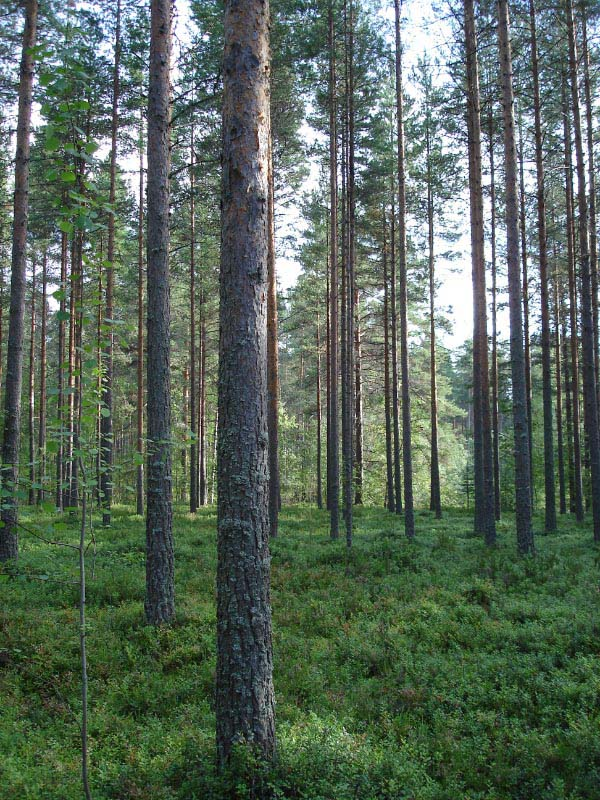
\includegraphics[height=0.65\textheight]{figures/PineForestJoensuu}\\
    {\small Scots pine forest in Joensuu.}
\end{frame}

\begin{frame}{Forest canopy}

    Looking upwards, circular `fish-eye' objective (180$^\circ$). May 15 and June 6 in Viikki.

    \centering
    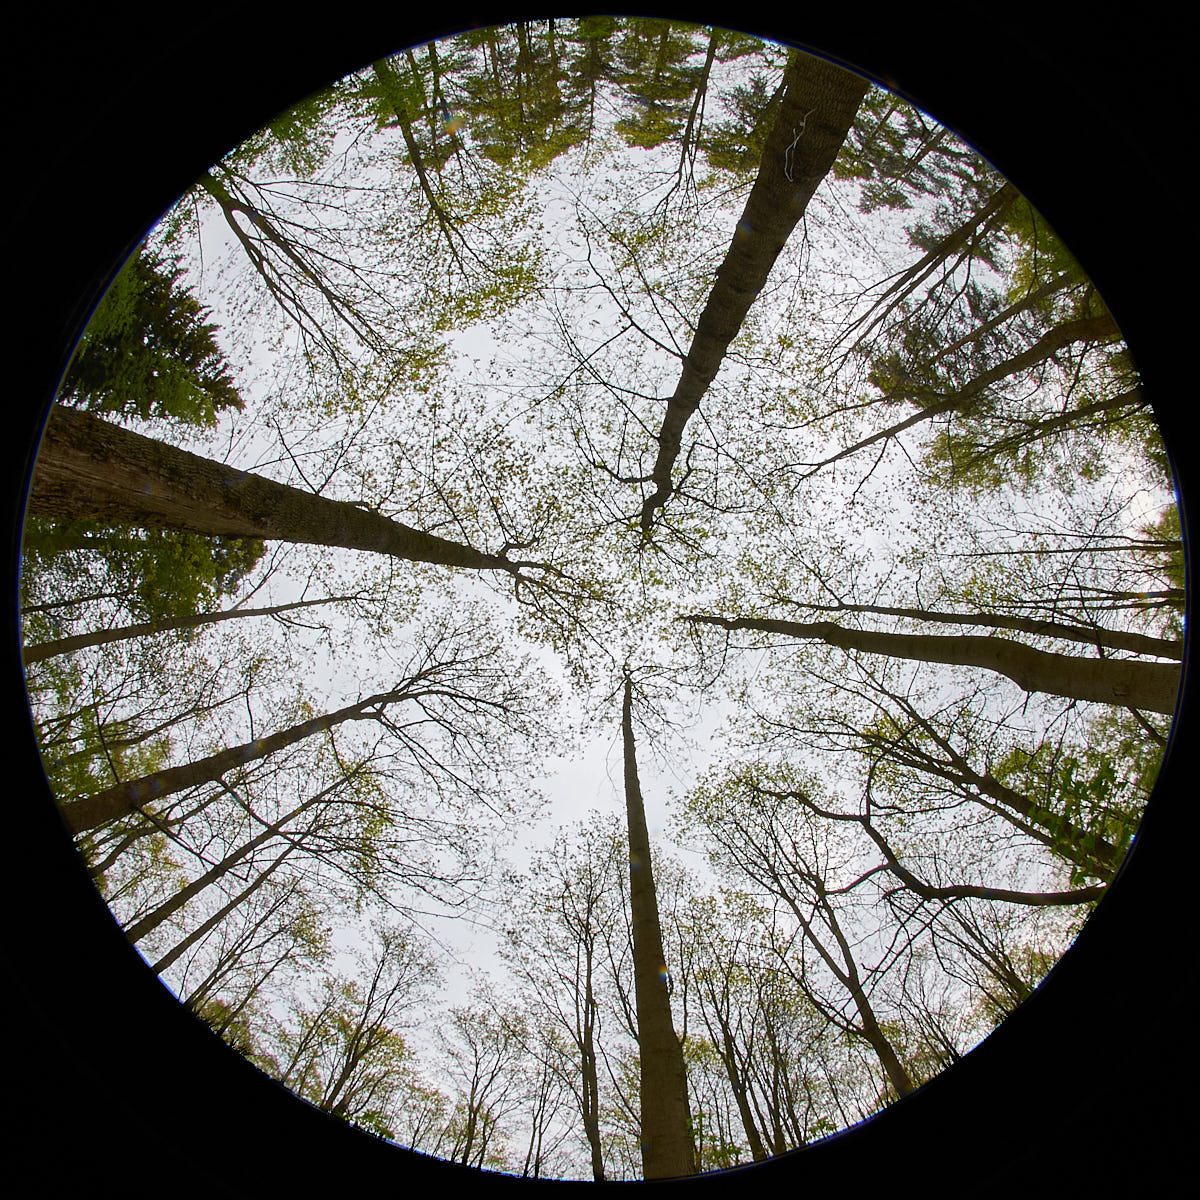
\includegraphics[width=0.45\textwidth]{photos/hemis-may-17}\hfil
    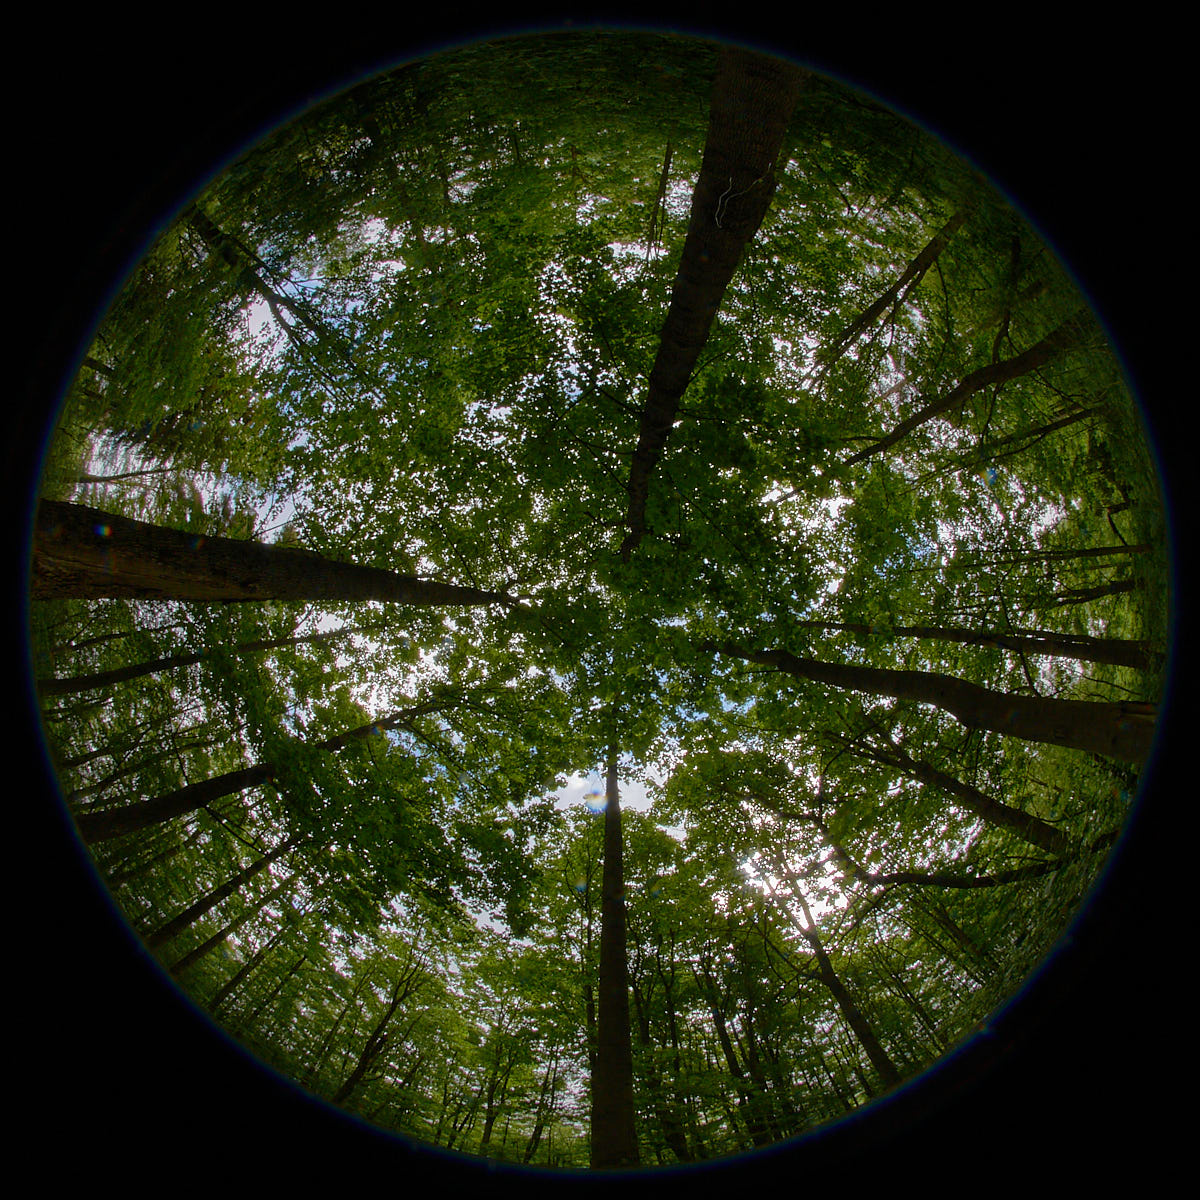
\includegraphics[width=0.45\textwidth]{photos/hemis-june-6}

    {\small Photos: T. M. Robson and S. Hartikainen.}
\end{frame}

\section{Radiation climatology}

\begin{frame}{Solar radiation as a resource}{Plant productivity and available radiation}
    \begin{itemize}
        \item Solar radiation is the source of energy for photosynthesis, but only
        absorbed light can be used.
        \item The yearly total of radiation depends on latitude and
        cloudiness.
        \item Arid regions tend to receive more sunlight, but there
        is little vegetation to use it because of lack of water.
    \end{itemize}
\end{frame}

\begin{frame}{Solar radiation as a resource}{Geographical variation in mean annual radiation}
    \centering
    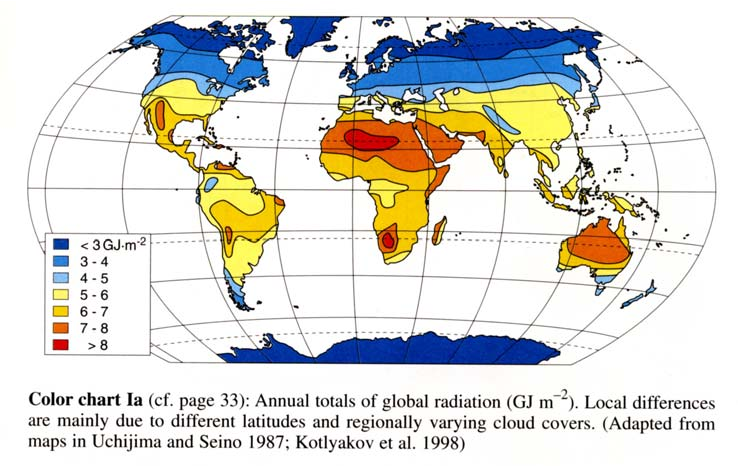
\includegraphics[width=0.8\textwidth]{figures/GlobalRadiationMap}\\
    {\small \autocite[From][]{Larcher2003}.}
\end{frame}

\begin{frame}{R:FR photon ratio (sunlight, no shade)}
    \centering
    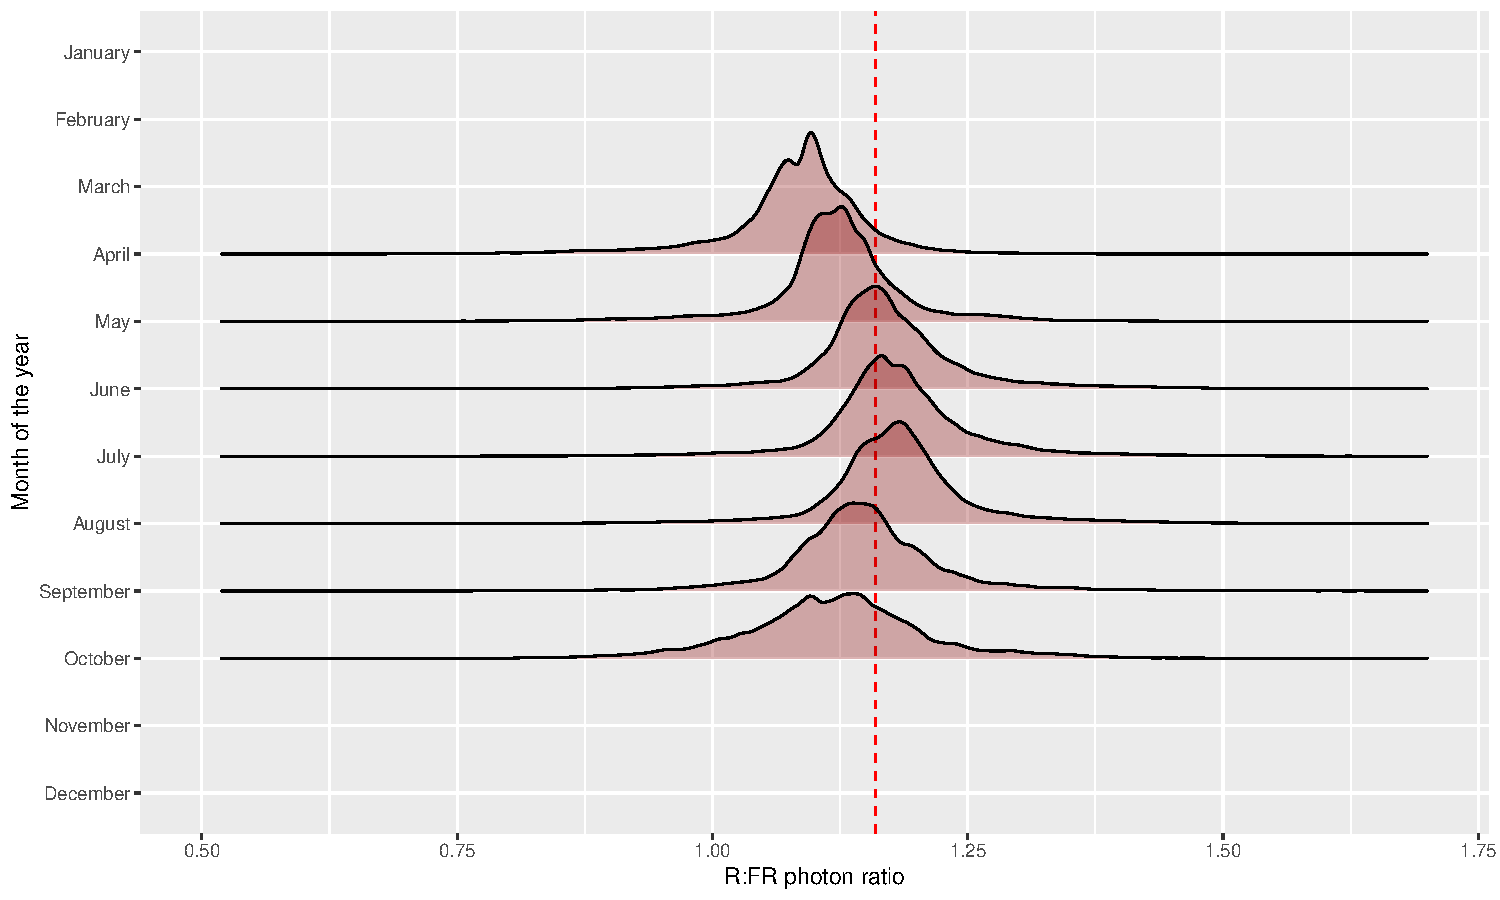
\includegraphics[width=0.8\textwidth]{figures/r-fr-dens-month-year-fig.pdf}\\
\end{frame}

  \section*{References}
  \nocite{Kotilainen2020,Durand2021,Durand2021a,Robson2019}
  \begin{frame}[t,allowframebreaks]
    \frametitle{References}
    \printbibliography
  \end{frame}

\end{document}
